\section{Spørgsmål 3}

\subsection{Fokuspunkter}
\begin{itemize}
	\item Hvordan er sammenhængen mellem Objekt Orientering og Relationsdatabaser.
	\begin{itemize}
		\item kom herunder ind på ligheder og forskelle på de to domæner.
	\end{itemize}
\end{itemize}

\subsection{Litteratur}
\begin{itemize}
	\item Database eLearning - \url{http://db.grussell.or/index.html}
	\begin{itemize}
		\item Kap. 2 - Advanced ER Mapping.
	\end{itemize}
	\item Database Modelling and Design
	\begin{itemize}
		\item Kap. 1 (s. 1 - 11)
		\item Kap. 3 (s. 35 - 53)
	\end{itemize}
	\item Agile Data Home Page - \url{http://www.agiledata.org/}
	\begin{itemize}
		\item Data Modeling (med undtagelse af part 3 sidste to emner(Normalize og Denormalize) samt part 5, 6 og 7).
		\item Mapping objects to RDBs (O/R mapping).
	\end{itemize}
\end{itemize}

\newpage

% must
\subsection{Hvordan er sammenhængen mellem Objekt Orientering og Relationsdatabaser?}

Objekter indeholder deres eget \textit{state} og \textit{relation}, samt komplekse værdier. En relationel database dekomponerer objekter ned til sorterede tupler af relationer.

Til arbejdet med OO og RDB, bruges en ORM\footnote{Object-Relation Mappeing} (Entity Framework), som oversætter fra en Relation Database til f.eks. C\# og vice versa.

En tabeller indgår rækker (tupler) og kolonner (attributter). 
Tuplerne definerer forskellige instanser af 'objektet'. Oversættes ét objekt til én tabel, får en \textit{1:1} sammenhæng mellem tabel og objekt.

\subsubsection{Objekt Orientering}
I OO-programmering tales der om instanser af klasser, som indeholder attributter.

\begin{itemize}
	\item Klasser er en brugerdefineret type.
	\item Indkapsling af data - private/public.
	\item Samarbejde gemmen pointer og referencer.
	\item Data manipuleres med metoder.
\end{itemize}

\subsubsection{Relationel Database}
I Relationelle databaser arbejdes der med entiteter, som indeholder attributter (kolonner).

\begin{itemize}
	\item Entiteter og relationer.
	\item Data manipuleres gemmen SQL statements.
	\item Relationer laves med primær- og fremmednøgler.
	\item Ingen metoden, kun data.
\end{itemize}

% must
\subsection{Ligheder og forskelle på de to domæner}

\begin{itemize}
	\item Klasse (som type) == Entity (som tabel). 
	\item Instans af klasse == Række i tabel.
	\item Medlemsdata bliver til kolonner/attributter i tabellen.
	\item Ingen metode i RDB, i stedet bruges \textit{Stored Procedures}, \textit{Functions} og \textit{Triggers}.
\end{itemize}

\subsubsection{Forskelle ved Arv}\label{sec:arv}
En klasse i OOP kan sagtens arve fra andre klasser, uden problemer. Der arves adfærd og medlemsdata. Dette kan en RDB ikke helt.

Der bruges super- og subklassen. Superklassen indeholder de 'generelle' attributter og subklassen er en specialisering af superklassen.

\begin{figure}[H]
\centering
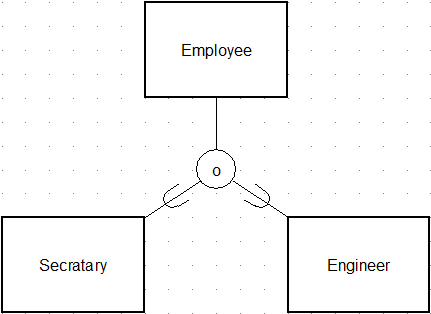
\includegraphics[width=0.5\linewidth]{figs/spm3/arv}
\caption{Arv i et ERD. }
\label{fig:arv}
\end{figure}

Specialisering kan ske \textit{overlapping} og \textit{disjoint}. 
Figur~\ref{fig:arv} viser \textit{overlapping} med 'o' i cirklen. Dette betyder at en \textit{Employee} \textbf{både} kan være en Ingeniør og en Sekretær.\\

Hvis det havde været et 'd' i stedet, ville specialiseringen være \textit{disjoint}. Dette ville betyde at en \textit{Employee} kan være Ingeniør \textbf{eller} Sekretær, altså ikke begge dele. 

\todo{Mere om hvad der sker med tabellerne ift. arv}

\subsubsection{Forskelle for Relationer}

\paragraph{1:1}

\begin{itemize}
	\item \textbf{OO}
	Brug af pointers/referencer.
	\item \textbf{DB}
	Laves med fremmed- og primærnøgle.
\end{itemize}

\paragraph{1:M}

\begin{itemize}
	\item \textbf{OO}
	Array med pointere eller Liste.
	\item \textbf{DB}
	'Mange'-siden har FK som er 'en'-sidens PK.
\end{itemize}

\paragraph{M:M}

\begin{itemize}
	\item \textbf{OO}
	Begge klasser indeholder array med pointere eller Liste.
	\item \textbf{DB}
	Ny tabel (weak entity) indføres mellem tabellerne. Denne indeholder flere FK som 'peger' tilbage på PK.
\end{itemize}

%Id/nøgler i db vs C\#. 
%
% pas på med brugen af entities. 
%
%entity i EF er noget der mapping in i ''den fysiske verden''.
%
%EF er et ORM, object relation management værktøj.
%
%Hele emnet kan ikke nås til eksamen, så vælg noget og tag det med, jt siger noget om arve-hierarki er godt. Hvor det implementeres med ER, UML og db konstruktion (ID PK/FK | Navn...)
%
%nedarvning i ER har ikke noget med arv at gøre, laves som en specialisering og generalisering.
